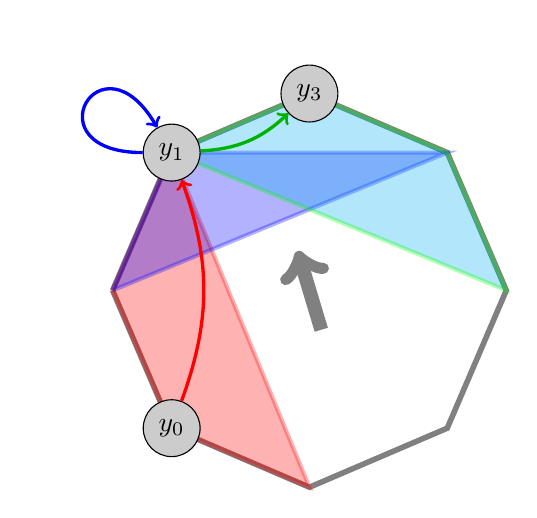
\begin{tikzpicture}[scale=0.5]
\coordinate (A1) at (-5, 0);
\coordinate (A2) at (-3.5, 3.5);
\coordinate (A3) at ( 0, 5);
\coordinate (A4) at ( 3.5, 3.5);
\coordinate (A5) at ( 5, 0);
\coordinate (A6) at ( 3.5,-3.5);
\coordinate (A7) at ( 0,-5);
\coordinate (A8) at (-3.5,-3.5);
\coordinate (O1) at ( 0.3,-1);
\coordinate (O2) at (-0.3,1);

\draw[line width=2pt  ,color=black!50]                       (A1) -- (A2) -- (A3) -- (A4) -- (A5) -- (A6) -- (A7) -- (A8) -- (A1);
\draw[line width=1.5pt,color=red     ,fill=red,opacity=0.3]  (A8) --(A1) -- (A2)  -- (A7) -- (A8);
\draw[line width=1.5pt,color=blue    ,fill=blue,opacity=0.3] (A1) -- (A2)  -- (A4) -- (A1);
\draw[line width=1.5pt,color=green    ,fill=cyan,opacity=0.3] (A2) -- (A3)  -- (A4) -- (A5) -- (A2);

\node[draw, fill=black!20,circle] (N1) at (A8) { $y_0$};
\node[draw, fill=black!20,circle] (N2) at (A2) { $y_1$};
\node[draw, fill=black!20,circle] (N3) at (A3) { $y_3$};

\path[very thick, ->,color=red]  (N1)  edge   [bend right=20]   (N2);
\path[very thick, ->,color=blue]  (N2)  edge   [out=180,in=120,looseness=10]   (N2);
\path[very thick, ->,color=green!70!black ]  (N2)  edge   [bend right=20]   (N3);
\path[line width=5.0pt, ->, black!50 ]  (O1)  edge  (O2);



%\draw (A1) -- (A4) -- (A3);
%\draw[dashed] (B1) -- (A2) -- (B2);
%\draw (B1) -- (A4) -- (B2);
%\draw (B1) -- (A1) -- (B2) -- (A3) --cycle;



\end{tikzpicture}
